\chapter{Lezione 20}
\label{chap:lezione_20}

\begin{flushright}
\textit{Data: 01/12/2025}
\end{flushright}

\section{Calcolo degli Integrali nei Diagrammi di Feynman}

Nelle lezioni precedenti abbiamo introdotto l'espansione perturbativa della funzione di correlazione a due punti $\langle \varphi(0) \varphi(x) \rangle$ in termini della costante di accoppiamento $g$. Abbiamo identificato i diagrammi di Feynman rilevanti all'ordine $g^2$.
L'obiettivo di questa lezione è calcolare esplicitamente il valore di questi diagrammi.

\noindent Nello spazio delle posizioni, questi calcoli coinvolgono integrali di prodotti di propagatori $G_0(x-y)$ che possono diventare estremamente lunghi e complessi da risolvere ("It's too long").
La strategia risolutiva standard consiste nel passare allo Spazio di Fourier (spazio dei momenti), dove le operazioni di convoluzione si trasformano in semplici prodotti. 

\noindent Ricordiamo che il propagatore libero in spazio di Fourier è dato da:

\begin{equation}
\tilde{G}_0(p) = \frac{1}{\mu + p^2}
\end{equation}

dove $\mu$ rappresenta la massa quadra e $p^2$ è il modulo quadro del momento. Le relazioni di trasformata sono:

\begin{equation}
G_0(x) = \int_{-\pi}^{\pi} \frac{d^D p}{(2\pi)^D} e^{i p \cdot x} \tilde{G}_0(p)
\end{equation}

\begin{equation}
\tilde{G}_0(p) = \int_{V} d^D x \, e^{-i p \cdot x} G_0(x)
\end{equation}

Inoltre, utilizzeremo l'identità della delta di Dirac in spazio $D$-dimensionale:

\begin{equation}
\delta^{(D)}(x) = \int_{-\pi}^{\pi} \frac{d^D p}{(2\pi)^D} e^{i p \cdot x}
\end{equation}

\newpage
\subsection{Il Diagramma ad una Bolla}

Consideriamo il diagramma connesso con una bolla:

\begin{equation*}
    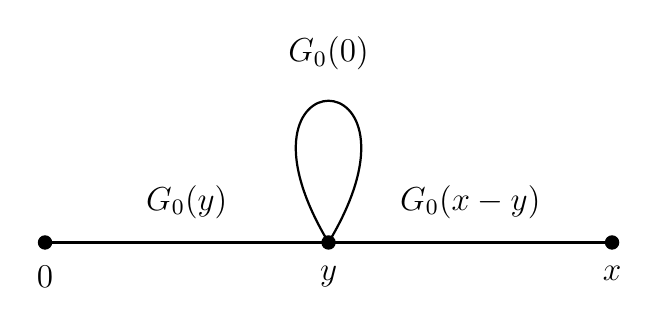
\begin{tikzpicture}[scale=1.2, baseline=(current bounding box.center)]
        % Definisco le coordinate per comodità e per distanziare i punti
        \coordinate (zero) at (0,0);
        \coordinate (y) at (3,0);   % Distanza aumentata a 3 unità
        \coordinate (x) at (6,0);   % Distanza totale 6 unità

        % Linee dei propagatori orizzontali
        % 'midway' centra la scritta, 'above=5pt' la distanzia dalla linea
        \draw[thick] (zero) -- node[midway, above=5pt] {\large $G_0(y)$} (y);
        \draw[thick] (y) -- node[midway, above=5pt] {\large $G_0(x-y)$} (x);
        
        % Vertici (pallini) e etichette dei punti (sotto)
        \filldraw [black] (zero) circle (2pt) node[below=5pt] {\large $0$};
        \filldraw [black] (x) circle (2pt) node[below=5pt] {\large $x$};
        \filldraw [black] (y) circle (2pt) node[below=5pt] {\large $y$};
        
        % Loop su y (Bolla)
        % Ho alzato i punti di controllo (1.8, 2.0) e (4.2, 2.0) per fare un arco ampio
        \draw[thick] (y) .. controls (1.8, 2.0) and (4.2, 2.0) .. (y);
        
        % Etichetta del loop posizionata ben sopra la bolla
        \node at (3, 2) {\large $G_0(0)$};
    \end{tikzpicture}
\end{equation*}

    
\noindent Nello spazio delle posizioni, il contributo $D_1$ associato a questo diagramma è un integrale sul vertice interno $y$:

\begin{equation}
D_1(x) = \int d^D y \, G_0(x-y) G_0(y) G_0(0) 
\end{equation}

Per semplicità, analizziamo la struttura base della convoluzione di due propagatori con un loop locale (che è costante nello spazio). Il termine cruciale è la convoluzione:

\begin{equation}
(G_0 * G_0)(x) = \int d^D y \, G_0(x-y) G_0(y)
\end{equation}

Sfruttiamo il \textbf{Teorema della Convoluzione}: la trasformata di Fourier di una convoluzione è il prodotto delle trasformate di Fourier.

\begin{equation}
\mathcal{F} \{ (f * g)(x) \} = \mathcal{F} \{ f(x) \} \cdot \mathcal{F} \{ g(x) \}
\end{equation}

\noindent Dimostriamolo esplicitamente inserendo le trasformate di Fourier nell'integrale spaziale:

\begin{equation}
\int d^D y \, G_0(x-y) G_0(y) = \int d^D y \int \frac{d^D p}{(2\pi)^D} e^{i p(x-y)} \tilde{G}_0(p) \int \frac{d^D q}{(2\pi)^D} e^{i q y} \tilde{G}_0(q)
\end{equation}

Raggruppiamo i termini dipendenti da $y$:

\begin{equation}
= \int \frac{d^D p}{(2\pi)^D} \int \frac{d^D q}{(2\pi)^D} e^{i p x} \tilde{G}_0(p) \tilde{G}_0(q) \left[ \int d^D y \, e^{i(q-p) \cdot y} \right]
\end{equation}

L'integrale in $dy$ genera una delta di Dirac:

\begin{equation}
\int d^D y \, e^{i(q-p) \cdot y} = (2\pi)^D \delta^{(D)}(q-p)
\end{equation}

Sostituendo la delta nell'espressione e integrando in $dq$:

\begin{equation}
= \int \frac{d^D p}{(2\pi)^D} \frac{1}{(2\pi)^D} (2\pi)^D \tilde{G}_0(p) \tilde{G}_0(p) e^{i p x} = \int \frac{d^D p}{(2\pi)^D} e^{i p x} \left[ \tilde{G}_0(p) \right]^2 = \mathcal{F}^{-1} \left[ \tilde{G}_0(p) \right]^2
\end{equation}

\noindent Quindi, nello spazio dei momenti, la convoluzione diventa:

\begin{tcolorbox}[colback=colorA!10, colframe=colorB!60!colorA,  title=\textbf{Diagramma ad una bolla}]
\begin{equation}
\tilde{D}_1(p) = \frac{1}{(2\pi)^D} \left[ \tilde{G}_0(p) \right]^2 \cdot \int d^Dq \; \tilde{G}_0(q)
\end{equation}
\end{tcolorbox}

\newpage
\subsection{Il Diagramma a Doppia Bolla}
Consideriamo il diagramma connesso di ordine $g^2$ costituito da due "tadpoles" (bolle) disgiunti posti sulla linea del propagatore.

\begin{equation*}
    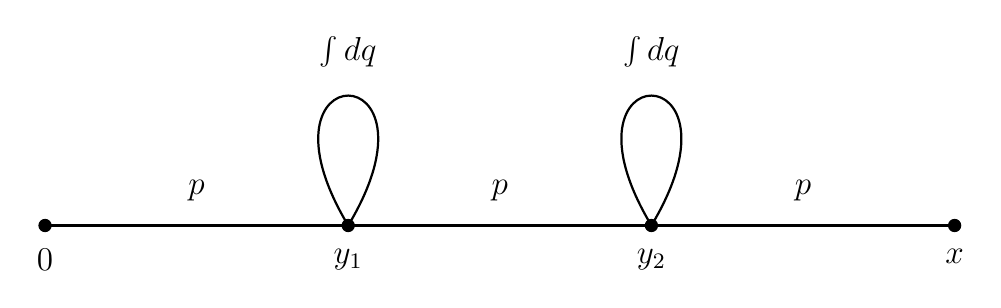
\begin{tikzpicture}[scale=1.1, baseline=(current bounding box.center)]
        % Definisco le coordinate: distanzio i punti di 3.5 unità per far stare tutto comodo
        \coordinate (zero) at (0,0);
        \coordinate (y1) at (3.5,0);
        \coordinate (y2) at (7.0,0);
        \coordinate (x) at (10.5,0);

        % --- Linee dei propagatori orizzontali ---
        % Segmento 0 -> y1
        \draw[thick] (zero) -- node[midway, above=5pt] {\large $p$} (y1);
        
        % Segmento y1 -> y2 (propagatore intermedio)
        \draw[thick] (y1) -- node[midway, above=5pt] {\large $p$} (y2);
        
        % Segmento y2 -> x
        \draw[thick] (y2) -- node[midway, above=5pt] {\large $p$} (x);
        
        % --- Vertici (pallini) e etichette dei punti (sotto) ---
        \filldraw [black] (zero) circle (2pt) node[below=5pt] {\large $0$};
        \filldraw [black] (y1) circle (2pt) node[below=5pt] {\large $y_1$};
        \filldraw [black] (y2) circle (2pt) node[below=5pt] {\large $y_2$};
        \filldraw [black] (x) circle (2pt) node[below=5pt] {\large $x$};
        
        % --- Loop su y1 (Prima Bolla) ---
        % Punti di controllo calcolati per creare un arco ampio che non tocchi le scritte
        \draw[thick] (y1) .. controls (2.3, 2.0) and (4.7, 2.0) .. (y1);
        \node at (3.5, 2) { \large $\int dq$};

        % --- Loop su y2 (Seconda Bolla) ---
        \draw[thick] (y2) .. controls (5.8, 2.0) and (8.2, 2.0) .. (y2);
        \node at (7.0, 2) { \large $\int dq$};
        
    \end{tikzpicture}
\end{equation*}


\noindent Questo diagramma coinvolge due vertici interni $y_1$ e $y_2$. La struttura nello spazio reale è una catena di convoluzioni moltiplicata per i loop locali:

\begin{equation}
D_2(x) = \underbrace{\int d^D y_1 \int d^D y_2 \, G_0(x-y_2) G_0(y_2-y_1) G_0(y_1)}_{\text{Linea Principale}} \times \underbrace{[G_0(0)]^2}_{\text{Loops}}
\end{equation}

\noindent Possiamo separare la parte relativa ai loop locali, che non dipende dalle coordinate di integrazione, portandola fuori dall'integrale. Ricordando che $G_0(0)$ in spazio dei momenti è un integrale su $q$:

\begin{equation}
= \left( \frac{1}{(2\pi)^D} \int \tilde{G}_0(q) d^D q \right)^2 \int d^D y_2 \int d^D y_1 \left( G_0(x-y_2) G_0(y_2-y_1) \right) G_0(y_1)
\end{equation}

\noindent Per risolvere l'integrale spaziale rimanente, riconosciamo la struttura di una convoluzione nidificata:
\begin{equation}
\int d^D y_2 \, G_0(x-y_2) \underbrace{\left[ \int d^D y_1 G_0(y_2-y_1) G_0(y_1) \right]}_{\text{Convoluzione interna}}
\end{equation}

\noindent Utilizziamo la trasformata di Fourier $\mathcal{F}$ e la sua inversa $\mathcal{F}^{-1}$.
L'integrale interno in $d^D y_1$ è una convoluzione tra la funzione $G_0(y_2 - y_1)$ e $G_0(y_1)$.
Possiamo quindi riscrivere l'integrale come:

\begin{equation}
\int d^D y_2 \mathcal{F}^{-1} \left\{ \mathcal{F} (G_0(x-y_2) G_0(y_2-y_1)) \cdot \mathcal{F}(G_0(y_1)) \right\}
\end{equation}


\noindent Procedendo con l'integrale esterno su $y_2$, riconosciamo che anche questo è una convoluzione, la seconda.
Applicando nuovamente il teorema della convoluzione, otteniamo il prodotto delle trasformate di Fourier di tre propagatori:

\begin{equation}
= \mathcal{F}^{-1} \left[ \mathcal{F}[G_0]^3 \right]
\end{equation}

Quindi, il risultato finale nello spazio dei momenti è dato dal prodotto del cubo del propagatore (dalla linea principale) per il quadrato dell'integrale di loop:

\begin{tcolorbox}[colback=colorA!10, colframe=colorB!60!colorA,  title=\textbf{Diagramma a Doppia Bolla}]
\begin{equation}
\tilde{D}_2(p)^{00} = \frac{1}{(2\pi)^D} \left[ \tilde{G}_0(p) \right]^3 \left( \int d^D q \, \tilde{G}_0(q) \right)^2
\end{equation}
\end{tcolorbox}

\newpage
\subsection{Il Diagramma a Cactus}

Consideriamo ora il diagramma a "Cactus".
In questo diagramma, abbiamo un vertice interno $y_1$ sulla linea principale, e un secondo vertice $y_2$ che si trova "sopra" il primo, formando un loop sopra un loop.

\begin{equation*}
    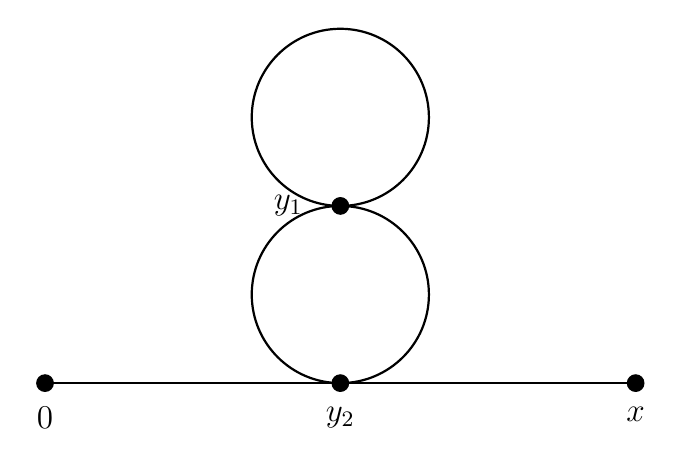
\begin{tikzpicture}[scale=1.5, baseline=(current bounding box.center)]
        % Coordinate
        \coordinate (zero) at (-2.5,0);
        \coordinate (x) at (2.5,0);
        \coordinate (y2) at (0,0);      % Vertice sulla linea principale (base del cactus)
        \coordinate (y1) at (0,1.5);    % Vertice intermedio (collo del cactus)

        % --- Linea Principale ---
        % Linea orizzontale passante per y2
        \draw[thick] (zero) -- node[midway, above=4pt] {} (y2);
        \draw[thick] (y2) -- node[midway, above=4pt] {} (x);
        
        % --- Loop Inferiore (Bolla tra y2 e y1) ---
        % Disegno come due archi che formano un cerchio di diametro 1.5
        % Centro ideale a (0, 0.75)
        \draw[thick] (y2) arc (-90:90:0.75); % Arco destro
        \draw[thick] (y2) arc (270:90:0.75); % Arco sinistro
        
        % --- Loop Superiore (Tadpole su y1) ---
        % Disegno come un cerchio completo tangente a y1
        % Centro a (0, 1.5 + 0.75) = (0, 2.25), Raggio 0.75
        \draw[thick] (0, 2.25) circle (0.75);
        
      
        % --- Vertici ---
        \filldraw [black] (zero) circle (2pt) node[below=5pt] {\large $0$};
        \filldraw [black] (x) circle (2pt) node[below=5pt] {\large $x$};
        \filldraw [black] (y2) circle (2pt) node[below=5pt] {\large $y_2$};
        \filldraw [black] (y1) circle (2pt) node[left=10pt] {\large $y_1$};
        
    \end{tikzpicture}
\end{equation*}

\noindent Nello spazio delle posizioni, la struttura è diversa dal caso precedente.
Abbiamo sempre una linea principale che passa per $y_1$, ma ora $y_2$ non è sulla linea principale; è connesso solo a $y_1$ tramite un loop. L'espressione associata a questo diagramma è:

\begin{equation}
\int d^D y_1 \int d^D y_2 \, G_0(x-y_2) G_0(y_2) G_0(y_1-y_2)^2 G_0(0)
\end{equation}

\noindent Possiamo portare fuori dall'integrale spaziale il termine $G_0(0)$ relativo al loop superiore, che è costante.
Esprimendolo in trasformata di Fourier come $\int \tilde{G}_0(q) d^D q$, l'espressione diventa:

\begin{equation}
= (2\pi)^{-D} \int_B \tilde{G}_0(q) d^D q \int d^D y_1 \int d^D y_2 \, G_{x2} G_{2} G_{21}^2
\end{equation}
abbiamo usato la notazione sintetica: $G_{x2} = G_0(x-y_2)$, $G_2 = G_0(y_2)$, $G_{21}~=~G_0(~y_1~-~y_2~)$

\noindent Per calcolare l'integrale rimanente, passiamo allo spazio dei momenti sostituendo ogni propagatore con la sua rappresentazione integrale di Fourier. Introduciamo i momenti $p_1, p_2, p_3, p_4$:

\begin{align*}
 =\int_V d^D y_1 \int_V d^D y_2 \int_B d^D p_1 \int_B d^D p_2 \int_B d^D p_3 \int_B d^D p_4 & \, e^{i p_1 (x-y_2)} \tilde{G}_0(p_1) e^{i p_2 y_2} \tilde{G}_0(p_2) \\ &\cdot e^{i p_3 (y_1-y_2)} \tilde{G}_0(p_3) e^{i p_4 (y_1-y_2)} \tilde{G}_0(p_4)
\end{align*}

\noindent Ora integriamo sulle variabili spaziali $y_1$ e $y_2$ per ottenere le funzioni Delta di conservazione del momento. L'integrale su $y_1$ isola i termini dipendenti da $y_1$ ($p_3$ e $p_4$):
\begin{equation}
\frac{\int d^D y_1}{(2\pi)^D} \longrightarrow \delta^{(D)}(p_4 - p_3)
\end{equation}


\noindent L'integrale su $y_2$ raccoglie tutti i momenti che entrano/escono da $y_2$:
\begin{equation}
\frac{\int d^D y_2}{(2\pi)^D} \longrightarrow \delta^{(D)}(-p_1 + p_2 + p_3 - p_4)
\end{equation}

\noindent Utilizzando le Delta per integrare sui momenti ridondanti, otteniamo il risultato finale.
Si noti che i momenti del loop inferiore ($p_3, p_4$) sono disaccoppiati dal momento esterno $p_1$ (che attraversa la linea principale come $p$).
L'espressione finale nello spazio dei momenti è data dal prodotto del propagatore esterno, del tadpole, e di un integrale di loop:

\begin{equation}
D_2^{8} = \mathcal{F}^{-1} \left\{ (2\pi)^{-D} \tilde{G}_0(p)^2 \int \frac{d^D q}{(2\pi)^D} \tilde{G}_0(q) \int \frac{d^D k}{(2\pi)^D} \tilde{G}_0(k)^2 \right\}
\end{equation}


\begin{tcolorbox}[colback=colorA!10, colframe=colorB!60!colorA,  title=\textbf{Diagramma a Cactus}]
\begin{equation}
\tilde{D}_2^8(p) = \frac{1}{(2\pi)^D} \left[ \tilde{G}_0(p) \right]^2 \cdot \int \frac{d^D q}{(2\pi)^D} \tilde{G}_0(q) \cdot \int \frac{d^D k}{(2\pi)^D} \tilde{G}_0(k)^2
\end{equation}
\end{tcolorbox}


\subsection{Il Diagramma Tramonto}

Consideriamo infine il diagramma irreducibile a due vertici $y_1, y_2$ connessi da tre linee interne.

\begin{equation*}
    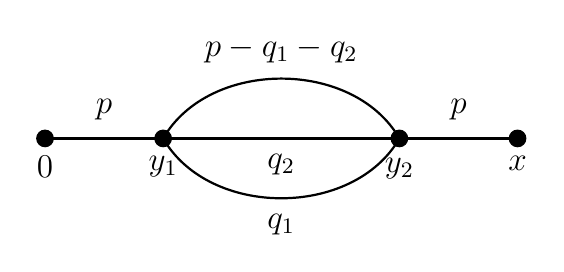
\begin{tikzpicture}[scale=1.5, baseline=(current bounding box.center)]
        \coordinate (zero) at (-2,0);
        \coordinate (y1) at (-1,0);
        \coordinate (y2) at (1,0);
        \coordinate (x) at (2,0);

        % Linee esterne
        \draw[thick] (zero) -- node[midway, above=3pt] {\large $p$} (y1);
        \draw[thick] (y2) -- node[midway, above=3pt] {\large $p$} (x);
        
        % Vertici
        \filldraw [black] (zero) circle (2pt) node[below=3pt] {\large $0$};
        \filldraw [black] (y1) circle (2pt) node[below=3pt] {\large $y_1$};
        \filldraw [black] (y2) circle (2pt) node[below=3.5pt] {\large $y_2$};
        \filldraw [black] (x) circle (2pt) node[below=3pt] {\large $x$};
        
        % Linee interne
        \draw[thick] (y1) -- node[midway, below=2pt] {\large $q_2$} (y2); 
        \draw[thick] (y1) to[bend left=60] node[midway, above=2pt] {\large $p-q_1-q_2$} (y2);
        \draw[thick] (y1) to[bend right=60] node[midway, below=2pt] {\large $q_1$} (y2);
    \end{tikzpicture}
\end{equation*}

\noindent Nello spazio delle posizioni:
\begin{equation}
D_{sun}(x) = \int d^D y_1 \int d^D y_2 \, G_0(x-y_1) \left[ G_0(y_1-y_2) \right]^3 G_0(y_2)
\end{equation}

\noindent Nello spazio dei momenti, la conservazione del quadrimpulso implica che la somma dei momenti sulle tre linee interne deve essere uguale al momento esterno $p$.
Se chiamiamo $q_1$ e $q_2$ due momenti di loop indipendenti, il terzo momento è fissato a $p - q_1 - q_2$.

L'espressione finale è:
\begin{tcolorbox}[colback=colorA!10, colframe=colorB!60!colorA,  title=\textbf{Diagramma a Cactus}]
\begin{equation}
\tilde{D}_{sun}(p) = \tilde{G}_0(p)^2 \int \frac{d^D q_1}{(2\pi)^D} \int \frac{d^D q_2}{(2\pi)^D} \tilde{G}_0(q_1) \tilde{G}_0(q_2) \tilde{G}_0(p - q_1 - q_2)
\end{equation}
\end{tcolorbox}


\noindent Questo diagramma è l'unico al secondo ordine che introduce una dipendenza non banale dal momento esterno $p$.

\newpage
\section{Regole Generali di Feynman}

Per calcolare sistematicamente i contributi perturbativi alla funzione di correlazione (in particolare la funzione a 2 punti $\langle \varphi(0)\varphi(x) \rangle$ o il propagatore completo $\tilde{G}(p)$), si applicano le seguenti regole generali, valide all'ordine $n$-esimo dello sviluppo perturbativo ($\mathcal{O}(g^n)$).

\begin{enumerate}
    \item \textbf{Linee Esterne:}
    Ad ogni linea esterna del diagramma è associato un momento $p$. Per la funzione di correlazione a 2 punti, questo contribuisce con un fattore pari al quadrato del propagatore libero:
    \begin{equation}
        \text{Fattore: } \tilde{G}_0(p)^2
    \end{equation}
    Questo fattore rappresenta i due "gambi" del diagramma che connettono la parte interna ai punti esterni 0 e $x$.

    \item \textbf{Linee Interne:}
    Ad ogni linea interna è associato un momento variabile $q_i$ che scorre in una data direzione.
    \begin{equation}
        \text{Fattore: } \tilde{G}_0(q_i)
    \end{equation}

    \item \textbf{Vertici:}
    Ad ogni vertice di interazione (dove si incontrano 4 linee nella teoria $\varphi^4$) deve essere conservato il momento totale. Questo è imposto da una funzione Delta di Dirac:
    \begin{equation}
        (2\pi)^D \delta^{(D)} \left( \sum p_{\text{in}} - \sum p_{\text{out}} \right)
    \end{equation}
    Ad ogni vertice è associato anche il fattore di accoppiamento  $-12g$.

    \item \textbf{Integrazione sui Loop:}
    All'ordine $\mathcal{O}(g^n)$, ci sono $n$ vertici e un certo numero di momenti interni liberi. Si deve integrare su tutti i momenti interni indipendenti (momenti di loop) $q_k$:
    \begin{equation}
        \int \frac{d^D q_k}{(2\pi)^D}
    \end{equation}
\end{enumerate}


\section{Irriducibilità a una Particella (1PI)}

Un concetto fondamentale per organizzare la serie perturbativa è quello di \textbf{Irriducibilità a una Particella} (One-Particle Irreducible, 1PI).

\begin{tcolorbox}[colback=yellow!25, colframe=yellow!75!orange, coltitle=black, title=\textbf{Definizione 1PI}]
Un diagramma si dice \textbf{1PI} se \textbf{non può} essere diviso in due diagrammi disconnessi tagliando una singola linea interna.
\end{tcolorbox}

Analizziamo alcuni esempi grafici per chiarire la distinzione:

\begin{itemize}
    \item \textbf{Diagramma 1PI (Setting Sun, singola bolla connessa, Cactus):}
    \begin{center}
    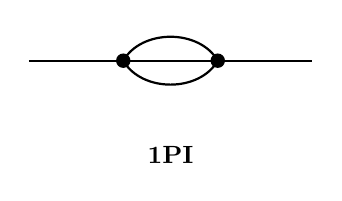
\begin{tikzpicture}[scale=1.2]
        \draw[thick] (-1.5,0) -- (-0.5,0); % Gamba sx
        \draw[thick] (0.5,0) -- (1.5,0);   % Gamba dx
        \filldraw [black] (-0.5,0) circle (2pt);
        \filldraw [black] (0.5,0) circle (2pt);
        % Linee interne
        \draw[thick] (-0.5,0) -- (0.5,0);
        \draw[thick] (-0.5,0) to[bend left=60] (0.5,0);
        \draw[thick] (-0.5,0) to[bend right=60] (0.5,0);
        \node at (0,-1) {\small \textbf{1PI}};
    \end{tikzpicture}
    \end{center}


    \item \textbf{Diagramma Riducibile (NON 1PI):}
    \begin{center}
    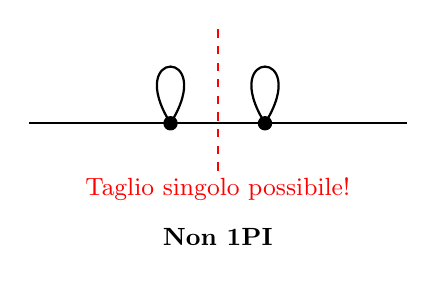
\begin{tikzpicture}[scale=1.2]
        \draw[thick] (-2,0) -- (2,0); % Linea base
        \filldraw [black] (-0.5,0) circle (2pt);
        \filldraw [black] (0.5,0) circle (2pt);
        % Bolle disgiunte
        \draw[thick] (-0.5,0) .. controls (-1.0,0.8) and (0.0,0.8) .. (-0.5,0);
        \draw[thick] (0.5,0) .. controls (0.0,0.8) and (1.0,0.8) .. (0.5,0);
        
        \draw[red, dashed, thick] (0, -0.5) -- (0, 1.0);
        \node[red] at (0, -0.7) {\small Taglio singolo possibile!};
        \node at (0,-1.2) {\small \textbf{Non 1PI}};
    \end{tikzpicture}
    \end{center}
   
\end{itemize}

\subsection{Sviluppo in Serie della Funzione di Correlazione}

Possiamo ora scrivere esplicitamente lo sviluppo perturbativo della funzione di correlazione a due punti completa $\langle \varphi(0)\varphi(x) \rangle$ (o equivalentemente del propagatore $\tilde{G}(p)$) sommando i contributi di tutti i diagrammi topologicamente distinti, pesati dai rispettivi fattori di simmetria e dalle costanti di accoppiamento.
La serie fino all'ordine $g^2$ è data da:

\begin{equation}
\langle \varphi(0)\varphi(x) \rangle = 1 + (-12g) D_1 + (144g^2) D_{2}^{00} + (144g^2) D_{2}^{8} + (96g^2) D_{2}^{sun} + O(g^3)
\label{eq:expansion_series}
\end{equation}


\begin{itemize}
    \item \textbf{Ordine 0:} Il propagatore libero (linea semplice).
    \item \textbf{Ordine $g$:} Il diagramma Tadpole (una bolla).
    \item \textbf{Ordine $g^2$:} Compaiono tre contributi distinti:
    \begin{enumerate}
        \item Double Scoop.
        \item Cactus.
        \item Setting Sun.
    \end{enumerate}
\end{itemize}

Ecco la rappresentazione diagrammatica corrispondente all'Equazione (\ref{eq:expansion_series}):

\begin{equation*}
    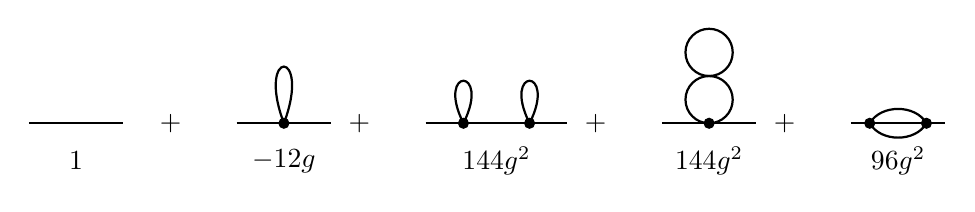
\begin{tikzpicture}[scale=1.2, baseline=(current bounding box.center)]
        % --- Termine 1 (Propagatore Libero) ---
        \draw[thick] (0,0) -- (1,0);
        \node at (0.5, -0.4) {$1$};
        
        \node at (1.5, 0) {$+$};
        
        % --- Termine 2 (Tadpole) ---
        \begin{scope}[shift={(2.2,0)}]
            \draw[thick] (0,0) -- (1,0);
            \filldraw (0.5,0) circle (1.5pt);
            \draw[thick] (0.5,0) .. controls (0.2, 0.8) and (0.8, 0.8) .. (0.5,0);
            \node at (0.5, -0.4) {$-12g$};
        \end{scope}
        
        \node at (3.5, 0) {$+$};
        
        % --- Termine 3 (Double Scoop - Due bolle disgiunte) ---
        \begin{scope}[shift={(4.2,0)}]
            \draw[thick] (0,0) -- (1.5,0);
            \filldraw (0.4,0) circle (1.5pt);
            \filldraw (1.1,0) circle (1.5pt);
            % Bolla 1
            \draw[thick] (0.4,0) .. controls (0.1, 0.6) and (0.7, 0.6) .. (0.4,0);
            % Bolla 2
            \draw[thick] (1.1,0) .. controls (0.8, 0.6) and (1.4, 0.6) .. (1.1,0);
            \node at (0.75, -0.4) {$144g^2$};
        \end{scope}
        
        \node at (6.0, 0) {$+$};
        
        % --- Termine 4 (Cactus - Bolle nidificate) ---
        \begin{scope}[shift={(6.7,0)}]
            \draw[thick] (0,0) -- (1,0);
            \filldraw (0.5,0) circle (1.5pt);
            % Loop inferiore
            \draw[thick] (0.5,0) arc (-90:270:0.25);
            % Loop superiore (attaccato sopra)
            \draw[thick] (0.5, 0.5) arc (-90:270:0.25);
            \node at (0.5, -0.4) {$144g^2$};
        \end{scope}
        
        \node at (8.0, 0) {$+$};
        
        % --- Termine 5 (Setting Sun) ---
        \begin{scope}[shift={(8.7,0)}]
            \draw[thick] (0,0) -- (1,0);
            \filldraw (0.2,0) circle (1.5pt);
            \filldraw (0.8,0) circle (1.5pt);
            % Linee interne
            \draw[thick] (0.2,0) to[bend left=60] (0.8,0);
            \draw[thick] (0.2,0) to[bend right=60] (0.8,0);
            \draw[thick] (0.2,0) -- (0.8,0);
            \node at (0.5, -0.4) {$96g^2$};
        \end{scope}
    \end{tikzpicture}
\end{equation*}

\subsection{Risommazione della Serie e Autoenergia}

Osservando la serie sopra, notiamo che alcuni diagrammi (come il Double Scoop e il Cactus) sono semplici ripetizioni o combinazioni di diagrammi di ordine inferiore.
Per organizzare meglio la serie, introduciamo il concetto di \textbf{diagramma amputato}.
Definiamo $\Sigma_1$ come il diagramma a una bolla "amputato", ovvero privato delle gambe esterne e dei fattori di accoppiamento esterni:

\begin{equation}
\Sigma_1^{\dots 0 \dots } \equiv \int \frac{d^D q}{(2\pi)^D} \tilde{G}_0(q)
\end{equation}


\noindent L'integrale $\Sigma_1$ è una costante (non dipende dal momento esterno $p$).
Possiamo ora riscrivere il propagatore completo $\tilde{G}_{\Omega}(p)$ sommando su tutte le possibili occorrenze di queste bolle lungo la linea di propagazione:

\begin{equation}
\tilde{G}_{\Omega}(p) = \tilde{G}_0(p) + \sum_{k=1}^{\infty} \tilde{G}_0(p) \left( -12g \tilde{G}_0(p) \Sigma_1 \right)^k + \dots
\end{equation}

\noindent Questa è una serie geometrica della forma $\sum x^k$ con ragione $x = -12g \tilde{G}_0(p) \Sigma_1$.
Sommando la serie otteniamo:

\begin{equation}
\tilde{G}_{\Omega}(p) = \tilde{G}_0(p) \left( \frac{1}{1 + 12g \tilde{G}_0(p) \Sigma_1} \right)
\end{equation}

\noindent Semplificando l'espressione:

\begin{equation}
\tilde{G}_{\Omega}(p) = \frac{1}{\tilde{G}_0(p)^{-1} + 12g \Sigma_1}
\end{equation}

\noindent Ricordando che l'inverso del propagatore libero è $\tilde{G}_0(p)^{-1} = p^2 + \mu$, arriviamo all'espressione finale risommata (al primo ordine di autoenergia):

\begin{tcolorbox}[colback=colorA!10, colframe=colorB!60!colorA,  title=\textbf{Propagatore Completo}]
\begin{equation}
\tilde{G}_{\Omega}(p) = \frac{1}{p^2 + \mu + 12g \Sigma_1}
\end{equation}
\end{tcolorbox}

\noindent Questa equazione mostra che l'effetto delle fluttuazioni quantistiche/termiche a questo ordine è semplicemente quello di spostare la massa (o la temperatura critica) del sistema:
\begin{equation}
\mu_{eff} = \mu + 12g \Sigma_1
\end{equation}

\section{Funzione di Correlazione a 4 Punti}

Consideriamo infine la funzione di correlazione a 4 punti $\langle \varphi(x_1)\varphi(x_2)\varphi(x_3)\varphi(x_4) \rangle_0$.
Nello sviluppo perturbativo, i diagrammi che contribuiscono a questa funzione possono essere raggruppati in 3 classi fondamentali:

\subsubsection{1. Diagrammi Completamente Disconnessi}
Questi diagrammi contengono parti (come le bolle di vuoto) che non sono connesse a nessuna delle linee esterne. Questi diagrammi vengono cancellati automaticamente dal denominatore della funzione di correlazione ($\mathcal{Z}$).

\subsubsection{2. Diagrammi Parzialmente Connessi (Riducibili)}
In questi diagrammi, tutte le parti sono connesse a qualche linea esterna, ma il diagramma complessivo è diviso in due o più componenti separate. Questi termini corrispondono al prodotto di funzioni a due punti (es. $\langle \varphi_1 \varphi_2 \rangle \langle \varphi_3 \varphi_4 \rangle$) e vengono rimossi prendendo la \textbf{parte connessa} della funzione di correlazione.

\subsubsection{3. Diagrammi Completamente Connessi}
Questa è la classe che contiene la vera informazione sull'interazione. Tutti e 4 i punti esterni sono connessi tra loro.

\begin{itemize}
    \item \textbf{Ordine 1:} Il diagramma a "X" (un singolo vertice).
    \begin{equation*}
        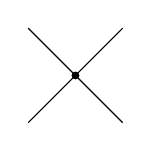
\begin{tikzpicture}[scale=0.6, baseline=(current bounding box.center)]
            \draw (-1,1) -- (1,-1);
            \draw (-1,-1) -- (1,1);
            \filldraw (0,0) circle (2pt);
        \end{tikzpicture}
    \end{equation*}
    
    \item \textbf{Ordine 2:} Diagrammi a loop che connettono i 4 punti.
    \begin{equation*}
        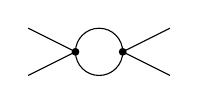
\begin{tikzpicture}[scale=0.6, baseline=(current bounding box.center)]
            \draw (-1.5,0.5) -- (-0.5,0);
            \draw (-1.5,-0.5) -- (-0.5,0);
            \draw (1.5,0.5) -- (0.5,0);
            \draw (1.5,-0.5) -- (0.5,0);
            \draw (0,0) circle (0.5);
            \filldraw (-0.5,0) circle (2pt);
            \filldraw (0.5,0) circle (2pt);
        \end{tikzpicture}
    \end{equation*}
    
\end{itemize}

